
\section{Empirical Evaluation}

\mlnote{Section needs an overhaul, rewrite, or removal}

%\mlnote{This section is still quite rough. I've commented out much of the text for now.}

%Here are some ides for what we could look at empirically: 
%\begin{itemize}
%\item Compare sampling techniques in each domain
%\item Quality of OOS as a function of the length of the match history $\tth$ (and time limits?)
%\item Robustness/sensitivity of $\delta_I$ and $\delta_{I,\tth}$ with observed convergence,
%\item Importance of ``retaining the tree'' from previous searches along the same match $z$ (suspected to be high)
%\item Performance comparisons (win rates and exploitability) between sampling techniques and some state-of-the-art
%algorithms in imperfect information search (ISMCTS, PIMC, MMCTS), 
%possibly also show exploitation / exploitability trade-offs as in RNash work
%\item (probably too much for this one paper) What if there are a sequence of multiple matches and we can reuse computation from 
%previous matches? 
%\item How does the story change with or without \{ incremental tree-building, targeting, retaining memory between searches \}
%\end{itemize}
%
% How does the story change: 
% - with/without targeting (as a function of delta)
% - with/without incremental tree-building
% - with/without remembering between moves

We now compare the head-to-head performance and exploitability 
of OOS and ISMCTS on two games. % with different sources of imperfect information. 
%We show the effects of targeting methods and $\delta$ values. 
%We start by describing each game, whose utilities are in $\{-1, 0, 1\}$. 

Liar's Dice, LD($D_1$,$D_2$), also known as Dudo, Perudo, and Bluff is a dice-bidding game. 
Each die has six sides with faces \epsdice{1} to \epsdice{5} and a star $\star$. 
Each player $i$ rolls $D_i$ of these dice and looks at them without showing them to their opponent. 
Each round, players alternate by bidding on the outcome of all dice in play until one player ``calls liar'', 
\ie claims that their opponent's latest bid does not hold.
A bid consists of a quantity of dice and a face value.  
A face of $\star$ is considered wild and counts as matching any other face.
To bid, the player must increase either the quantity or face value of the current 
bid (or both). The losing player discards a number of dice equal to how many dice were missing 
to have a valid bid. The players continue until one player has no more dice.

Imperfect Information II-Goofspiel($N$) is a two-player card game where each player is
given a private hand of bid cards with values $1$ to $N$. A different
deck of $N$ point cards is placed face up in a stack 
On their turn, each player bids for the top point card by 
choosing a single card in their hand. 
The highest bidder gets the point card and adds the point total to their score, discarding
the points in the case of a tie. 
This is repeated $N$ times and the winner is the player with the highest score.
In, II-Goofspiel the players only discover who won or lost a bid but not the bid cards played.
Also, we assume the point-stack is strictly increasing: 1, 2, $\ldots N$.

%Phantom Tic-Tac-Toe (PTTT) is played on a 3-by-3 board, 
%initially empty, where the goal is to claim three squares along the same row, column, or diagonal. 
%However, in PTTT, players' actions are private. 
%Each turn, a player attempts to take a square of their choice. 
%If they fail due to the opponent having taken that square on a previous turn, the same player 
%keeps trying to take an alternative square until they succeed. 
%Players are not informed about how many attempts the opponent made before succeeding. 
%The game ends immediately if there is ever a connecting line of squares belonging to the same player. 
%The winner receives a payoff of $+1$, while the losing player receives $-1$. 

We will focus our experiments on LD(1,1) and II-Goofspiel(6). While these games are considered small by 
search algorithm standards, it is still possible to compute best response strategies to measure exploitability, 
allowing us to show the observed convergence of the strategies
produced by OOS. We include preliminary results in LD(2,2). 

To improve performance against irrational play, we use a more explorative regret matching, 
$\sigma^{T+1}_\gamma(I,a) = \gamma/|A(I)| + (1-\gamma) \sigma^{T+1}(I,a)$, with $\gamma = 0.01$. 
While this could effect convergence, we observe in our experiments that exploitability 
decreases as search time increases.  

\subsection{Head-to-Head vs. Exploitability} 

\begin{figure}[t!]
\begin{center}
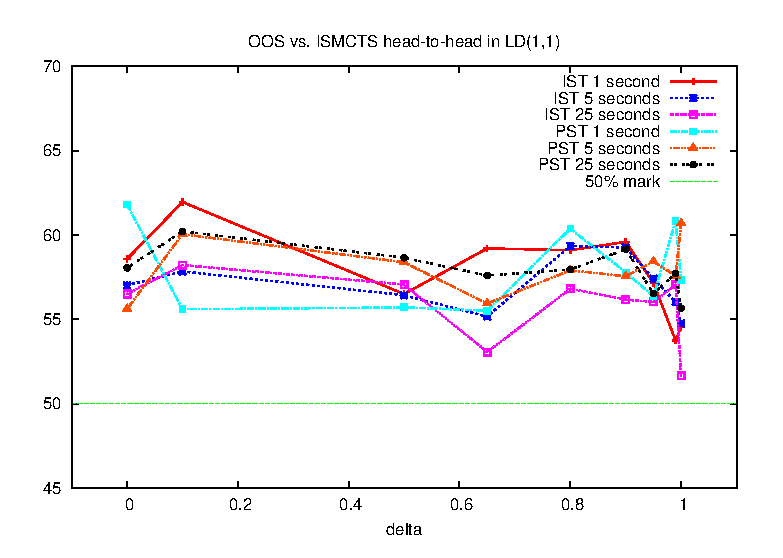
\includegraphics[scale=0.55]{plots/ismcts-oos-perf} \\
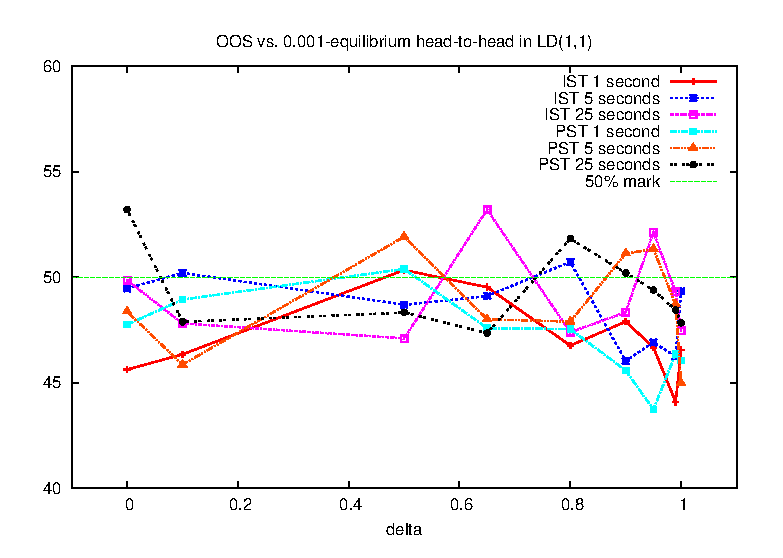
\includegraphics[scale=0.55]{plots/eq-oos-perf} \\
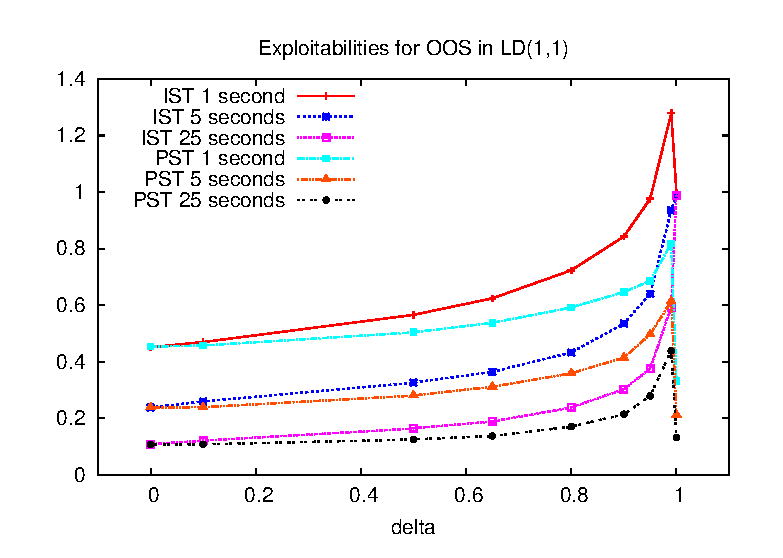
\includegraphics[scale=0.55]{plots/oos-expl} \\
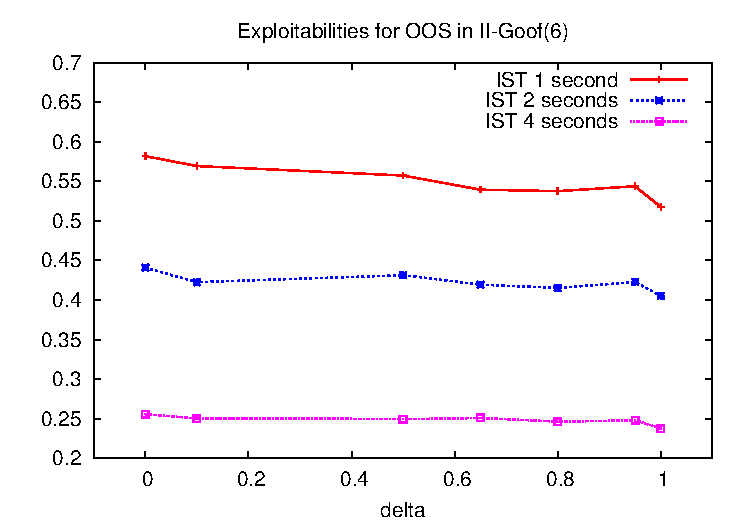
\includegraphics[scale=0.55]{plots/goof-expl} \\
\caption{Results for OOS in LD(1,1). From top: win rate (\%) of OOS vs. ISMCTS, win rate (\%) of 
OOS vs. a 0.001-equilibrium, approximate $\epsilon_{\sigma}$ using aggregate method in LD(1,1) 
and II-Goofpiel(6).  }
\label{fig:results}
\end{center}
\end{figure}

%Here are some first results for performance and/or exploitability analysis of the algorithms. 
%Note that unless otherwise stated, memory is retained and not cleared between successive searches
%(which has no effect in ISMCTS).
%\mlnote{I have played against the ISMCTS strategy and I believe it's converging to a particular 
%pure (and bad) strategy.}

%We evaluate head-to-head performance by simulating several games of each algorithm against the other
%and counting wins and losses. 

In games like Poker and Liar's Dice, it is often critical to play in such a way that the opponent 
cannot easily infer the private information. This explains partly why CFR-based methods have 
enjoyed so much success in the offline approach. 
In the online setting, however, since the tree is built incrementally, only partial strategies
are produced. 
We are unaware of any methods for assessing the worst-case exploitability of strategies 
produced by an online search algorithm. 
We therefore propose two new methods to approximate the exploitability of the produced strategies. 

In the offline setting, measuring exploitability can be done by a recursive walk of the game 
tree using expectimax. In online search, the algorithm computes only 
a partial strategy. 
The first \defword{full stitching} method 
enumerates each $I \in \cI_i$ in topologically-sorted order starting at the root, 
%tries to capture as closely as possible the distributions that would be computed 
%for each $I$ if they were reached in a match: 
running a search from $I$ re-using only the information computed in previous searches from ancestors of $I$, saving the 
distribution computed at $I$, and passing down the state of memory only for children of $I$. 
We do not save changes made to ancestors when searching at $I$ to ensure 
a fair comparison between OOS and ISMCTS. Full stitching provides the best representation of a full strategy
that would eventually be produced by OOS since it builds distributions at each information set in the 
same way as OOS would if they were reached during play.
However, full-stitching requires $|\cI|$ searches and memory, which is impractical on large games. 

We also propose a the multi-match \defword{aggregate method}. 
This method first creates a global (accumulating) strategy data structure for each player type and generates a 
set of matches $M$. Then, each $m \in M$ is simulated invoking the appropriate search algorithm at each observed 
$I$ along $m$. 
Since $m$ is predetermined, the choice made by the search algorithm is discarded, but the information computed 
(visit counts in ISMCTS, $s_I$ in OOS) is added into the global strategy data structure belonging to the player
who searched. 
For a fair comparison, the first $I$ reached along each $m$ aggregates all the information gained in the search 
but for future $I'$, only the information collected in each $I''$ reachable by $I'$ is aggregated.
Note that it is safe to combine the information in this way: in ISMCTS the actions chosen and visits are independent of 
how $I'$ was reached. In OOS, the accumulating $s_I$ values of two converging $\epsilon$-equilibrium average 
strategies can be combined due to linearity of expected utility. 

%a the \defword{partial stitching} method which does the same as full stitching to a fixed depth from the root, except also 
%retains values from children information sets reached by the searches started along the frontier of the depth limit.
% Probably will ditch this single-match method when partial stitching is working.
%And the \defword{single-match} method: this simply runs several matches and saves all values from each $I$ searched (as well as all of its reachable
%children information sets) search, overwriting previously saved values as necessary. 
 

In our experiments ISMCTS uses $C = 2$; tuning shows that the $C$ value does not 
affect the performance. 
In II-Goofspiel(6) we run searches for 1, 2, and 4 seconds.
As there are no public actions, we only compare IST in II-Goofspiel. 
Over a range of values for $\delta$ and all time settings, there was no statistically significant
winner in head-to-head matches between IST and ISMCTS. 
Exploitability is shown in Figure~\ref{fig:results}. 
For reference, the exploitability values of ISMCTS was 0.95, 0.96, 0.91 for search times of 
1, 2, and 4 seconds. We observe that exploitability generally 
decreases as search time increases and changes little as $\delta$ increases, with its 
lowest points at $\delta = 1$. 
This result was surprising, and we suspect it is due OOS benefiting from the reuse of 
values from previous searches in the same match. 

In LD(1,1), we try searches for 1, 5, and 25 seconds. 
When played against a uniform random player, among all values for delta and time settings, 
IST wins 79.2-86.7\% and PST wins 78.6-84.0\%, with a non-noticeable differences across $\delta$ values. 
ISMCTS beat uniform random 79.8-82.4\% at 1, 5, and 25 seconds. 
Upon further inspection, ISMCTS very quickly converges to the same strategy every time: as first player, 
with a weak roll ($r = \epsdice{1}, \epsdice{2},$ or \epsdice{3}) it bids 2-$r$ in the hope that by chance the
opponent has the same roll because if it did not, the second player would have a winning response most of the time.
On a roll of $r = \epsdice{4}$ or $r = \epsdice{5}$ it always bids 1-$r$ because it wins most of time. Either way, as 
second player ISMCTS selects responses based on the same reasoning, inducing the first player's roll based on their
first bid. This also explains the relative exploitability values in Table~\ref{tbl:fullstitching}: the first player
plays overly safely and hence is hard to exploit, meanwhile the second player best-responds to an expected pure first 
player strategy, which makes it highly exploitable. 
Our exploitability experiments shows a similar skewed first vs. second player effect in II-Goofspiel. 

Results for OOS variants on LD(1,1) are shown in Figure~\ref{fig:results}. Firstly, in head-to-head performance 
we notice OOS wins 55-60\% of games against ISMCTS, results for $\delta \in \{ 0.1, 0.8, 0.9 \}$ seem somewhat 
consistent across variants and time settings, with varied effects for $\delta > 0.9$. 
Against the 0.001-equilibrium strategy, 
$\delta = 0.5, 0.65$ seems the most robust across variants and time settings, with varied effects when $\delta > 0.9$.
Exploitability of ISMCTS strategies computed by the multi-match method was 0.88, 0.82, 0.79 at search times of 
1, 2, and 25 seconds. There are some clear trends for the exploitability of OOS strategies. 
First, there is an observed decrease in exploitability as time increases, independent of $\delta$. 
When $\delta$ is varied at the same time setting, the exploitability of the global strategy increases with $\delta$. 
Then, when $\delta = 1$ every time setting for IST converges to the same highly-exploitable point, illustrating the 
theoretical problems with full targeting manifesting in practice. 
Interestingly, this is not the case for PST, where $\delta = 1$ is actually always the best-case scenario. 
In Liar's Dice, this is sensible because there is no reason to believe that any histories outside the public subgame 
will effect the decisions being made when in the public subgame. 
The sudden drop from $\delta = 0.99$ to $1$ could be caused by the fact that as $\delta$ increases the 
variance of the importance-sampling corrections of the off-match samples grows; when $\delta = 1$ the 
sampled counterfactual values may be biased, but have much lower variance. 
PST is less affected than IST by the targeting and appears to have lower exploitability. 
For each method and all values of $\delta$: increasing the search time decreases exploitability. 
The exploitability values from Table~\ref{tbl:fullstitching} also show this trend. 

We performed one head-to-head experiment consisting of 500 games of PST($\delta = 0.8$) vs. ISMCTS, in LD(2,2)
with 25 seconds of search time per move. 
PST won 256 games, showing a competitive promise on 
this much larger game with roughly 352 million information sets. 

%Finally, inspired by~\cite{Auger11Multiple}, we started an initial investigation of OOS and ISMCTS in Phantom Tic-Tac-Toe. 
%We noticed that the mixed distribution obtained by normalizing the visit counts of ISMCTS was producing a 
%similar distribution as OOS on the second-player's first action. As in the Rock, Paper, Scissors
%example~\cite{Shafiei09}, we designed a biased version that gave higher payoff if the final line 
%included a side. This modification led to OOS and ISMCTS producing two distinctly different distributions at the second 
%player's first action. 

\begin{table}
{\small
\begin{center}
\begin{tabular}{ccccc}
Algorithm     & Time & $\epsilon_1$ & $\epsilon_2$ & $\epsilon_\sigma$ \\
\hline
ISMCTS        & 1s   & 0.235  & 0.574  & 0.808 \\
IST           & 1s   & 0.337  & 0.311  & 0.648 \\
PST           & 1s   & 0.203  & 0.211  & 0.414 \\
\hline
ISMCTS        & 5s   & 0.251  & 0.548  & 0.799 \\
IST           & 5s   & 0.229  & 0.295  & 0.524 \\
PST           & 5s   & 0.148  & 0.125  & 0.273 \\
\hline
\end{tabular}
\caption{LD(1,1) exploitability using full-stitching, $\delta = 0.9$.} 
\label{tbl:fullstitching}
\end{center}
}
\end{table}
